\documentclass[aspectratio=169,11pt]{beamer}
\usepackage[utf8]{inputenc}
\usepackage[T1]{fontenc}
\usepackage[brazilian]{babel}
\usepackage{amsmath,booktabs,graphicx,array}
% Figuras pré-compiladas em figuras/. Dados e falas documentados no roteiro.
% Recompilar figuras: powershell -File figuras/compilar-figuras.ps1
\usetheme{Singapore}
\title[PHVD-APS -- Apresentação final]{Planejamento de Visitas Domiciliares na APS}
\subtitle{Prioridades, rotas e replanejamento}
\author{Fabio Cieslak, Tobias Marion e Vitor Feijo}
\date{INF99003 -- Projeto 2 -- Grupo A\\Apresentação Final -- 09/10/2026}
\definecolor{ink}{HTML}{202124}
\definecolor{muted}{HTML}{666666}
\definecolor{blue}{RGB}{30,80,160}
\definecolor{green}{RGB}{30,130,60}
\definecolor{red}{RGB}{190,60,60}
\definecolor{light}{HTML}{E8E8E8}
\definecolor{amber}{HTML}{B68432}
\setbeamercolor{normal text}{fg=ink,bg=white}
\setbeamersize{text margin left=8mm,text margin right=8mm}
\setbeamertemplate{navigation symbols}{}
\setbeamercovered{transparent}
\setbeamertemplate{footline}[frame number]
\newcommand{\bigtext}[1]{{\fontsize{24.88}{30}\selectfont #1\par}}
\newcommand{\smallnote}[1]{\par\vspace{2mm}{\fontsize{8}{10}\selectfont\color{muted}#1\par}}
\newcommand{\labeltext}[1]{{\color{muted}\small #1}}
\begin{document}
% 01
\begin{frame}[c]
\titlepage
\end{frame}
% 02
\section{Problema}
\begin{frame}{O problema de planejamento}
\centering
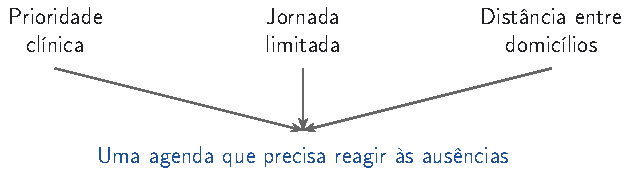
\includegraphics{figuras/02-problema-planejamento.pdf}
\end{frame}
% 03
\begin{frame}{Hipótese}
\centering
{\large Prioridade + horizonte móvel + busca local}
\par\vspace{7mm}{\large $\Downarrow$}
\par\vspace{7mm}\large{Menor atraso,\\com custo operacional controlado}
\end{frame}
% 04
\begin{frame}{Literatura e decisões de projeto}
\vspace{2mm}
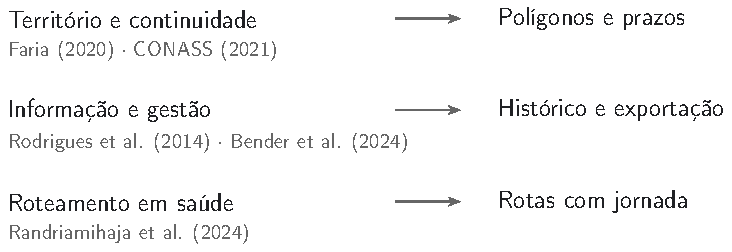
\includegraphics{figuras/04-literatura-decisoes.pdf}
\smallnote{Revisão de oito trabalhos. Nosso recorte acrescenta comparação de estratégias e replanejamento após falhas.}
\end{frame}
% 05
\begin{frame}{O que foi feito no projeto}
\centering
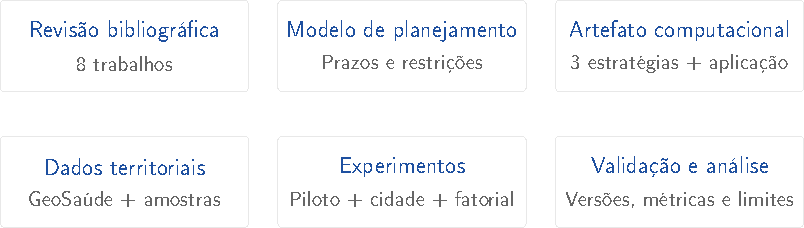
\includegraphics{figuras/05-realizacoes-projeto.pdf}
\end{frame}
% 06
\section{Modelo}
\begin{frame}{Modelo de planejamento}
\begin{columns}[c]
\column{.49\textwidth}
{\large Prazo = última visita + intervalo\par}
\vspace{6mm}\labeltext{$N$ dias úteis no horizonte}
\par\vspace{3mm}\labeltext{$A$ dias corridos de antecipação}
\par\vspace{6mm}{\large Deslocamento + visitas\\$\leq$ jornada da equipe}
\column{.49\textwidth}
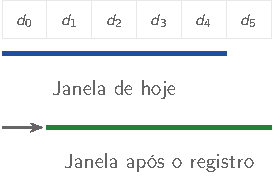
\includegraphics{figuras/06-horizonte-movel.pdf}
\end{columns}
\smallnote{Dias úteis esquemáticos. Restrições verificadas: território, disponibilidade, jornada e unicidade do paciente por rota.}
\end{frame}
% 07
\section{Artefato}
\begin{frame}{Artefato computacional}
\centering
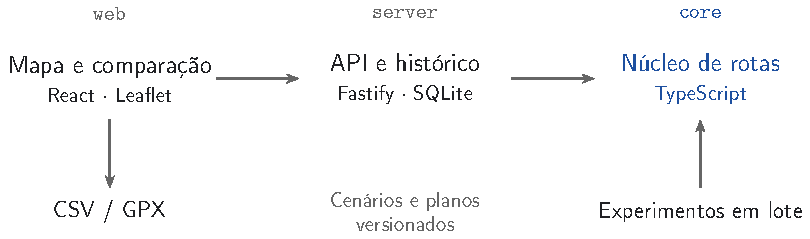
\includegraphics{figuras/07-arquitetura-artefato.pdf}
\end{frame}
% 08
\begin{frame}{Território, pacientes e uma rota}
\begin{columns}[c]
\column{.61\textwidth}\centering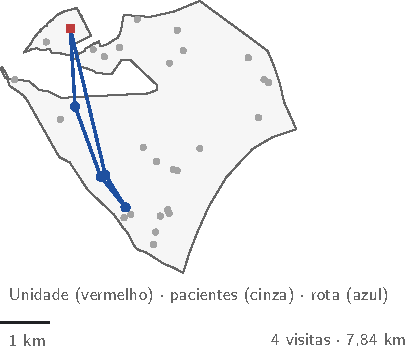
\includegraphics{figuras/08-mapa-restinga.pdf}
\column{.37\textwidth}
{\large US Restinga\par}
\vspace{4mm}\labeltext{Contorno GeoSaúde real}
\par\vspace{2mm}\labeltext{30 pacientes sintéticos}
\par\vspace{6mm}{\large Selecionar $\to$ amostrar\\$\to$ planejar $\to$ comparar}
\par\vspace{6mm}\labeltext{Registro de visitas + exportação}
\end{columns}
\smallnote{Exemplo gerado pelo núcleo: primeiro dia não vazio, 4,5 km/h, jornada de 240 min. Traços em linha reta.}
\end{frame}
% 09
\section{Métodos}
\begin{frame}{Três estratégias comparáveis}
\centering
{\large
\begin{tabular}{@{}>{\raggedright\arraybackslash}m{.28\textwidth}@{\hspace{5mm}}>{\raggedright\arraybackslash}m{.64\textwidth}@{}}
\textcolor{red}{Urgência} & Prioriza atraso acumulado e necessidade clínica\\[7mm]
\textcolor{green}{Vizinho próximo} & Escolhe a visita elegível com menor deslocamento\\[7mm]
\textcolor{blue}{Principal} & Constrói rotas, melhora trajetos e recupera prioridades
\end{tabular}}
\vspace{8mm}\par\labeltext{Mesmos pacientes, calendário, jornada e matriz de custos}
\smallnote{A melhoria intra-rota 1.5-opt está habilitada nas três estratégias nos experimentos apresentados.}
\end{frame}
% 10
\begin{frame}{Heurística principal: versão final}
\centering
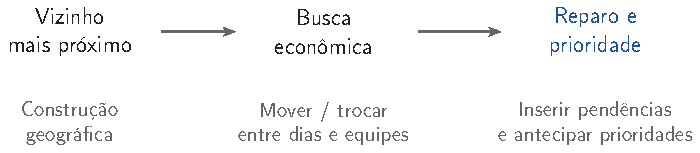
\includegraphics{figuras/10-heuristica-principal.pdf}
\vspace{8mm}\par{\large 1.5-opt em cada rota + limites de jornada}
\smallnote{A busca controla caminhada; a recuperação de visitas adicionais pode aumentar a distância total.}
\end{frame}
% 11
\begin{frame}{O que acontece quando a visita falha?}
\centering
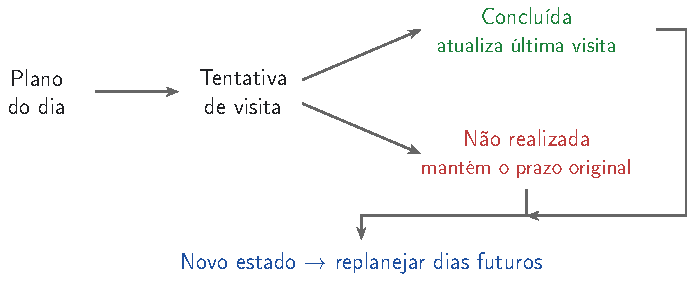
\includegraphics{figuras/12-replanejamento-ausencias.pdf}
\smallnote{Uma visita ausente conta deslocamento, permanece pendente e nunca é presumida como concluída.}
\end{frame}
% 12
\section{Experimentos}
\begin{frame}{Dois estudos complementares}
\begin{columns}[T]
\column{.48\textwidth}{\large Porto Alegre\par}
\vspace{5mm}{\fontsize{35.83}{42}\selectfont\color{blue}132}\par\labeltext{territórios reais}
\par\vspace{5mm}30 pacientes · 22 dias úteis
\par\vspace{2mm}1 amostra por território
\par\vspace{4mm}\textbf{1.188 simulações}
\column{.48\textwidth}{\large Fatorial na Restinga\par}
\vspace{5mm}{\fontsize{35.83}{42}\selectfont\color{blue}5}\par\labeltext{fatores, com três níveis}
\par\vspace{5mm}Pacientes · área · horizonte
\par\vspace{2mm}Vencidas · falhas · 3 sementes
\par\vspace{4mm}\textbf{2.187 simulações}
\end{columns}
\smallnote{Três estratégias; falhas de 0\%, 5\% e 10\% por tentativa; uma equipe de 240 min/dia; sorteios comuns por paciente e data.}
\end{frame}
% 13
\begin{frame}{Porto Alegre: maior resposta pronta}
\begin{columns}[c]
\column{.65\textwidth}
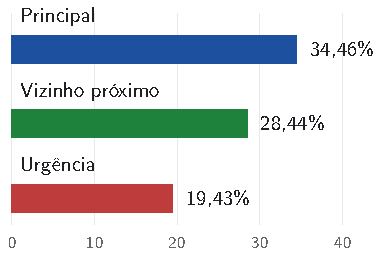
\includegraphics{figuras/15-resposta-pronta-porto-alegre.pdf}
\column{.32\textwidth}{\fontsize{24.88}{31}\selectfont\color{blue}\mbox{+6,02 p.p.}}\par
\vspace{4mm}{\large +21,2\% relativo}\par
\vspace{4mm}\labeltext{ante o vizinho próximo}
\par\vspace{7mm}\labeltext{Cobertura: 99,81\%\\vs. 99,72\%}
\end{columns}
\smallnote{Médias das 132 regiões e três taxas de falha, com peso igual. Demanda e perfis clínicos sintéticos.}
\end{frame}
% 14
\begin{frame}{O ganho tem custos e limites}
\centering
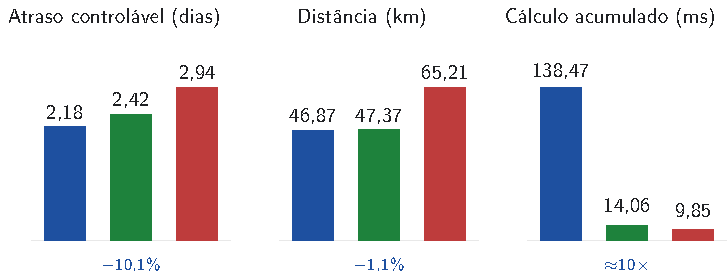
\includegraphics{figuras/16-custos-limites.pdf}
\par\vspace{5mm}{\small\textcolor{blue}{\rule{3mm}{2mm}} Principal\quad\textcolor{green}{\rule{3mm}{2mm}} Vizinho próximo\quad\textcolor{red}{\rule{3mm}{2mm}} Urgência}
\smallnote{Cada painel usa escala própria e base zero. Variações ante o vizinho. Tempo do horizonte simulado, dependente da máquina.}
\end{frame}
% 15
\begin{frame}{O ganho permanece com ausências}
\begin{columns}[c]
\column{.58\textwidth}
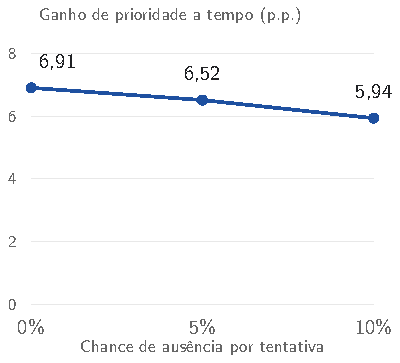
\includegraphics{figuras/17-ganho-ausencias.pdf}
\column{.37\textwidth}{\fontsize{35.83}{38}\selectfont\color{blue}283 / 396}\par
\labeltext{vitórias em resposta pronta}
\par\vspace{5mm}87 empates · 26 derrotas
\par\vspace{7mm}\labeltext{Distância maior em\\163 dos 396 pares}
\end{columns}
\smallnote{Porto Alegre, principal vs. vizinho próximo. Mesma ausência quando ambos visitam o mesmo paciente na mesma data.}
\end{frame}
% 16
\begin{frame}{Fatorial: o ganho varia com a demanda}
\begin{columns}[c]
\column{.55\textwidth}
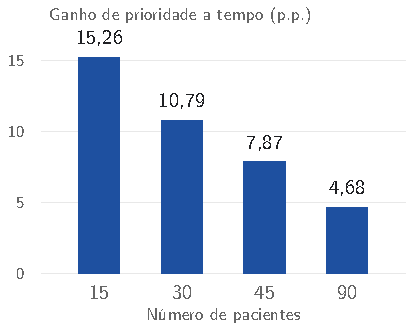
\includegraphics{figuras/18-fatorial-demanda.pdf}
\column{.42\textwidth}{\fontsize{29.86}{36}\selectfont\color{blue}+6,64 p.p.}\par
\labeltext{ganho médio em 729 pares}
\par\vspace{5mm}580 vitórias · 111 empates\par38 derrotas
\par\vspace{6mm}\labeltext{Distância: 334 derrotas\\Com 10\% de falha: +0,25 km}
\end{columns}
\smallnote{Principal vs. vizinho. Médias marginais sobre os outros fatores e três sementes. Área 0,5$\times$/2$\times$ é sintética.}
\end{frame}
% 17
\section{Conclusão}
\begin{frame}{Limites da evidência}
\vspace{4mm}
\begin{tabular}{@{}p{.44\textwidth}p{.49\textwidth}@{}}
{\large Pacientes sintéticos} & Perfis e ausências simulados\\[6mm]
{\large Distância Haversine} & Ruas e barreiras não avaliadas\\[6mm]
{\large Amostras controladas} & Uma equipe; poucas sementes\\[6mm]
{\large Comparação descritiva} & Sem superioridade universal
\end{tabular}
\smallnote{Eficiência simulada do algoritmo. Os resultados não medem benefício clínico na população.}
\end{frame}
% 18
\begin{frame}[c]{Conclusão}
\centering\bigtext{Melhor resposta às prioridades\\na avaliação simulada}
\vspace{8mm}{\large Menor atraso médio · caminhada média próxima}
\par\vspace{4mm}{\large Mais cálculo · vantagem variável entre cenários}
\vspace{9mm}\par\labeltext{Artefato reutilizável + experimentos reproduzíveis}
\end{frame}
% 19
\begin{frame}{Trabalhos futuros}
\vspace{3mm}
\begin{tabular}{@{}p{.25\textwidth}p{.67\textwidth}@{}}
{\large Ruas} & Avaliar o algoritmo com a matriz OSRM a pé\\[6mm]
{\large Campo} & Demanda e jornadas observadas; piloto com equipes\\[6mm]
{\large Generalização} & Mais sementes, territórios e múltiplas equipes\\[6mm]
{\large Método} & Pesos, ablações, Pareto e referência exata pequena
\end{tabular}
\smallnote{A integração OSRM já existe na aplicação; falta avaliar seus efeitos no protocolo experimental.}
\end{frame}
% 20
\begin{frame}{Referências}
\begin{columns}[T]
\column{.49\textwidth}
{\fontsize{8.2}{9.6}\selectfont
\textbf{Barros, Aquino e Souza (2022).} \emph{Evolução da estrutura e resultados da Atenção Primária à Saúde no Brasil entre 2008 e 2019.} Ciência \& Saúde Coletiva.\par\vspace{2mm}
\textbf{Matta e Morosini (s.d.).} \emph{Atenção Primária à Saúde.} Dicionário da Educação Profissional em Saúde, EPSJV/Fiocruz.\par\vspace{2mm}
\textbf{Faria (2020).} \emph{A territorialização da Atenção Básica à Saúde do Sistema Único de Saúde do Brasil.} Ciência \& Saúde Coletiva, 25(11), 4521--4530.\par\vspace{2mm}
\textbf{Randriamihaja et al. (2024).} \emph{Combining OpenStreetMap mapping and route optimization algorithms to inform the delivery of community health interventions at the last mile.} PLOS Digital Health, 3(11), e0000621.
}
\column{.49\textwidth}
{\fontsize{8.2}{9.6}\selectfont
\textbf{Rodrigues et al. (2014).} \emph{A atenção primária à saúde na coordenação das redes de atenção: uma revisão integrativa.} Ciência \& Saúde Coletiva, 19(2), 343--352.\par\vspace{2mm}
\textbf{CONASS (2021).} \emph{A Atenção Primária à Saúde no SUS: avanços e ameaças.} CONASS Documenta, n. 38, Brasília.\par\vspace{2mm}
\textbf{Pinto e Rocha (2015).} \emph{Inovações na Atenção Primária em Saúde: o uso de ferramentas de tecnologia de comunicação e informação para apoio à gestão local.} Ciência \& Saúde Coletiva.\par\vspace{2mm}
\textbf{Bender et al. (2024).} \emph{O uso de Tecnologias de Informação e Comunicação em Saúde na Atenção Primária à Saúde no Brasil, de 2014 a 2018.} Ciência \& Saúde Coletiva, 29(1), e19882022.
}
\end{columns}
\smallnote{Dados territoriais: GeoSaúde / Porto Alegre, Território Base (jul./2025).}
\end{frame}
% 21
\begin{frame}[plain,c]
\centering\bigtext{Obrigado!}
\end{frame}
\end{document}
